% law of log|zeta(0.7+it)| vs random Euler product (generated by a script).
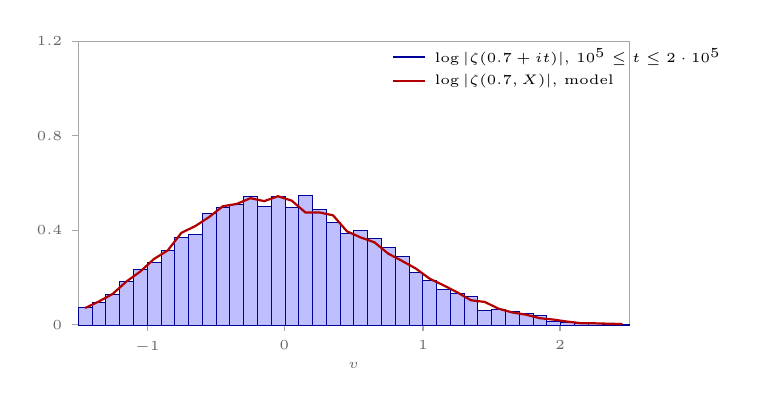
\begin{tikzpicture}[x=1cm,y=1cm]
\draw[black!35] (0,0) rectangle (7.00,3.60);
\draw[black!35] (0.88,0)--(0.88,-0.08) node[below,font=\tiny,black!60]{$-1$};
\draw[black!35] (2.62,0)--(2.62,-0.08) node[below,font=\tiny,black!60]{$0$};
\draw[black!35] (4.38,0)--(4.38,-0.08) node[below,font=\tiny,black!60]{$1$};
\draw[black!35] (6.12,0)--(6.12,-0.08) node[below,font=\tiny,black!60]{$2$};
\draw[black!35] (0,0.00)--(-0.08,0.00) node[left,font=\tiny,black!60]{$0$};
\draw[black!35] (0,1.20)--(-0.08,1.20) node[left,font=\tiny,black!60]{$0.4$};
\draw[black!35] (0,2.40)--(-0.08,2.40) node[left,font=\tiny,black!60]{$0.8$};
\draw[black!35] (0,3.60)--(-0.08,3.60) node[left,font=\tiny,black!60]{$1.2$};
\node[below,font=\tiny,black!60] at (3.50,-0.35) {$v$};
\filldraw[blue!25,draw=blue!60!black,line width=0.2pt] (0.000,0) rectangle (0.175,0.218);
\filldraw[blue!25,draw=blue!60!black,line width=0.2pt] (0.175,0) rectangle (0.350,0.285);
\filldraw[blue!25,draw=blue!60!black,line width=0.2pt] (0.350,0) rectangle (0.525,0.391);
\filldraw[blue!25,draw=blue!60!black,line width=0.2pt] (0.525,0) rectangle (0.700,0.548);
\filldraw[blue!25,draw=blue!60!black,line width=0.2pt] (0.700,0) rectangle (0.875,0.700);
\filldraw[blue!25,draw=blue!60!black,line width=0.2pt] (0.875,0) rectangle (1.050,0.788);
\filldraw[blue!25,draw=blue!60!black,line width=0.2pt] (1.050,0) rectangle (1.225,0.948);
\filldraw[blue!25,draw=blue!60!black,line width=0.2pt] (1.225,0) rectangle (1.400,1.109);
\filldraw[blue!25,draw=blue!60!black,line width=0.2pt] (1.400,0) rectangle (1.575,1.151);
\filldraw[blue!25,draw=blue!60!black,line width=0.2pt] (1.575,0) rectangle (1.750,1.418);
\filldraw[blue!25,draw=blue!60!black,line width=0.2pt] (1.750,0) rectangle (1.925,1.494);
\filldraw[blue!25,draw=blue!60!black,line width=0.2pt] (1.925,0) rectangle (2.100,1.527);
\filldraw[blue!25,draw=blue!60!black,line width=0.2pt] (2.100,0) rectangle (2.275,1.630);
\filldraw[blue!25,draw=blue!60!black,line width=0.2pt] (2.275,0) rectangle (2.450,1.503);
\filldraw[blue!25,draw=blue!60!black,line width=0.2pt] (2.450,0) rectangle (2.625,1.636);
\filldraw[blue!25,draw=blue!60!black,line width=0.2pt] (2.625,0) rectangle (2.800,1.488);
\filldraw[blue!25,draw=blue!60!black,line width=0.2pt] (2.800,0) rectangle (2.975,1.651);
\filldraw[blue!25,draw=blue!60!black,line width=0.2pt] (2.975,0) rectangle (3.150,1.463);
\filldraw[blue!25,draw=blue!60!black,line width=0.2pt] (3.150,0) rectangle (3.325,1.306);
\filldraw[blue!25,draw=blue!60!black,line width=0.2pt] (3.325,0) rectangle (3.500,1.166);
\filldraw[blue!25,draw=blue!60!black,line width=0.2pt] (3.500,0) rectangle (3.675,1.206);
\filldraw[blue!25,draw=blue!60!black,line width=0.2pt] (3.675,0) rectangle (3.850,1.103);
\filldraw[blue!25,draw=blue!60!black,line width=0.2pt] (3.850,0) rectangle (4.025,0.982);
\filldraw[blue!25,draw=blue!60!black,line width=0.2pt] (4.025,0) rectangle (4.200,0.866);
\filldraw[blue!25,draw=blue!60!black,line width=0.2pt] (4.200,0) rectangle (4.375,0.664);
\filldraw[blue!25,draw=blue!60!black,line width=0.2pt] (4.375,0) rectangle (4.550,0.567);
\filldraw[blue!25,draw=blue!60!black,line width=0.2pt] (4.550,0) rectangle (4.725,0.454);
\filldraw[blue!25,draw=blue!60!black,line width=0.2pt] (4.725,0) rectangle (4.900,0.406);
\filldraw[blue!25,draw=blue!60!black,line width=0.2pt] (4.900,0) rectangle (5.075,0.367);
\filldraw[blue!25,draw=blue!60!black,line width=0.2pt] (5.075,0) rectangle (5.250,0.188);
\filldraw[blue!25,draw=blue!60!black,line width=0.2pt] (5.250,0) rectangle (5.425,0.203);
\filldraw[blue!25,draw=blue!60!black,line width=0.2pt] (5.425,0) rectangle (5.600,0.170);
\filldraw[blue!25,draw=blue!60!black,line width=0.2pt] (5.600,0) rectangle (5.775,0.145);
\filldraw[blue!25,draw=blue!60!black,line width=0.2pt] (5.775,0) rectangle (5.950,0.124);
\filldraw[blue!25,draw=blue!60!black,line width=0.2pt] (5.950,0) rectangle (6.125,0.048);
\filldraw[blue!25,draw=blue!60!black,line width=0.2pt] (6.125,0) rectangle (6.300,0.036);
\filldraw[blue!25,draw=blue!60!black,line width=0.2pt] (6.300,0) rectangle (6.475,0.024);
\filldraw[blue!25,draw=blue!60!black,line width=0.2pt] (6.475,0) rectangle (6.650,0.018);
\filldraw[blue!25,draw=blue!60!black,line width=0.2pt] (6.650,0) rectangle (6.825,0.006);
\filldraw[blue!25,draw=blue!60!black,line width=0.2pt] (6.825,0) rectangle (7.000,0.003);
\draw[red!70!black,thick] (0.088,0.213) -- (0.262,0.296) -- (0.438,0.392) -- (0.613,0.550) -- (0.787,0.675) -- (0.963,0.836) -- (1.138,0.945) -- (1.312,1.169) -- (1.488,1.254) -- (1.662,1.368) -- (1.838,1.506) -- (2.013,1.535) -- (2.188,1.608) -- (2.363,1.571) -- (2.538,1.633) -- (2.712,1.577) -- (2.888,1.425) -- (3.062,1.428) -- (3.238,1.390) -- (3.413,1.188) -- (3.587,1.110) -- (3.763,1.048) -- (3.938,0.904) -- (4.113,0.812) -- (4.288,0.715) -- (4.462,0.587) -- (4.638,0.503) -- (4.812,0.414) -- (4.988,0.312) -- (5.163,0.291) -- (5.337,0.206) -- (5.513,0.157) -- (5.688,0.129) -- (5.863,0.084) -- (6.038,0.066) -- (6.212,0.041) -- (6.388,0.020) -- (6.562,0.019) -- (6.738,0.014) -- (6.913,0.010);
\draw[blue!60!black,thick] (4.00,3.40)--(4.40,3.40) node[right,font=\tiny,black]{$\log|\zeta(0.7+it)|$, $10^5\le t\le2\cdot10^5$};
\draw[red!70!black,thick] (4.00,3.10)--(4.40,3.10) node[right,font=\tiny,black]{$\log|\zeta(0.7,X)|$, model};
\end{tikzpicture}
